\section{Produto Misto}

\subsection{Definição}

Chama-se \textit{produto misto} dos vetores 
\[
  \vec{u} = x_1 \vec{i} + y_1 \vec{j} + z_1 \vec{k}, \quad
  \vec{v} = x_2 \vec{i} + y_2 \vec{j} + z_2 \vec{k}, \quad
  \vec{w} = x_3 \vec{i} + y_3 \vec{j} + z_3 \vec{k}
\]
(tomados nesta ordem) ao número real $(\vec{u} \cdot (\vec{v} \times \vec{w}))$.

O produto misto de $\vec{u}$, $\vec{v}$ e $\vec{w}$ também é indicado por:
\[
  \det(\vec{u}, \vec{v}, \vec{w}) \quad \text{ou} \quad 
  \begin{vmatrix}
    x_1 & y_1 & z_1 \\
    x_2 & y_2 & z_2 \\
    x_3 & y_3 & z_3
  \end{vmatrix}
\]

Tendo em vista que:
\[
  \vec{v} \times \vec{w} = 
  \begin{vmatrix}
    \vec{i} & \vec{j} & \vec{k} \\
    x_2 & y_2 & z_2 \\
    x_3 & y_3 & z_3
  \end{vmatrix}
  = (y_2 z_3 - y_3 z_2)\vec{i} - (x_2 z_3 - x_3 z_2)\vec{j} + (x_2 y_3 - x_3 y_2)\vec{k}
\]

temos:
\[
  \vec{u} \cdot (\vec{v} \times \vec{w}) = 
  x_1(y_2 z_3 - y_3 z_2) - y_1(x_2 z_3 - x_3 z_2) + z_1(x_2 y_3 - x_3 y_2)
\]

e, portanto:
\[
  \vec{u} \cdot (\vec{v} \times \vec{w}) = 
  \begin{vmatrix}
    x_1 & y_1 & z_1 \\
    x_2 & y_2 & z_2 \\
    x_3 & y_3 & z_3
  \end{vmatrix}
  \tag{1}
\]

\subsection{Propriedades do Produto Misto}

As propriedades do produto misto decorrem, em sua maioria, das propriedades dos
determinantes.

\subsubsection*{I. Troca de Sinal}

O produto misto $(\vec{u}, \vec{v}, \vec{w})$ muda de sinal ao trocarmos a
posição de dois vetores.

Em relação ao exemplo anterior, em que $(\vec{u}, \vec{v}, \vec{w}) = 27$,
teríamos:
\[
  (\vec{v}, \vec{u}, \vec{w}) = -27 \quad (\text{permuta de } \vec{u} \text{ e } \vec{v})
\]
\[
  (\vec{w}, \vec{v}, \vec{u}) = -27 \quad (\text{permuta de } \vec{u} \text{ e } \vec{w})
\]
\[
  (\vec{u}, \vec{w}, \vec{v}) = -27 \quad (\text{permuta de } \vec{v} \text{ e } \vec{w})
\]
Se em qualquer um desses três últimos produtos efetuarmos nova permutação de
dois vetores, o produto misto resultante volta a ser 27.

Portanto, se em relação ao produto misto $(\vec{u}, \vec{v}, \vec{w})$ ocorrer:
\begin{itemize}
  \item uma permutação – haverá troca de sinal;
  \item duas permutações – não altera o valor.
\end{itemize}

Resulta dessa propriedade que os sinais $\cdot$ e $\times$ podem ser permutados,
ou seja:
\[
  (\vec{u}, \vec{v}, \vec{w}) \cdot (\vec{u}, \vec{v}, \vec{w}) = (\vec{v}, \vec{w}, \vec{u}) = (\vec{w}, \vec{u}, \vec{v}) = (\vec{u}, \vec{v}, \vec{w}) = \vec{u} (\vec{v}, \vec{w}) 
\]

\subsubsection*{II. Propriedade de Linearidade}

\[
  (\vec{u}, \vec{v}, \vec{w}) + (\vec{x}, \vec{v}, \vec{w}) = (\vec{u} + \vec{x}, \vec{v}, \vec{w})
\]
\[
  (\vec{u}, \vec{v}, \vec{w}) + (\vec{u}, \vec{v}, \vec{w}) = (\vec{u}, \vec{v}, \vec{w})
\]

\subsubsection*{III. Produto Misto e Escalares}

\[
  \alpha (\vec{u}, \vec{v}, \vec{w}) = (\alpha \vec{u}, \vec{v}, \vec{w}) = (\vec{u}, \alpha \vec{v}, \vec{w}) = (\vec{u}, \vec{v}, \alpha \vec{w})
\]

\subsubsection*{IV. Produto Misto e Vetores Coplanares}

O produto misto $(\vec{u}, \vec{v}, \vec{w}) = 0$ se, e somente se, os três
vetores forem coplanares.

Admitindo-se que $(\vec{u}, \vec{v}, \vec{w}) = 0$, ou seja,
\[
  (\vec{u}, \vec{v}, \vec{w}) \cdot (\vec{v} \times \vec{w}) = 0,
\]
conclui-se que:
\[
  (\vec{v} \times \vec{w}) \perp \vec{u}.
\]

Por outro lado, no estudo do produto vetorial vimos que o vetor $\vec{v} \times
\vec{w}$ é também ortogonal a $\vec{v}$ e $\vec{w}$. Assim, como $\vec{v} \times
\vec{w}$ é ortogonal aos três vetores $\vec{u}$, $\vec{v}$ e $\vec{w}$, estes
são coplanares (Figura~\ref{fig:fig4.1}).

\begin{figure}[H]
  \begin{center}
    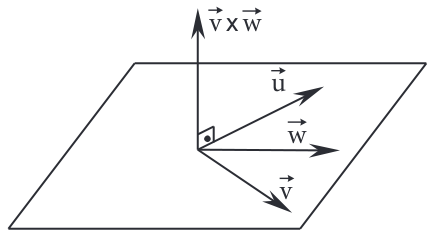
\includegraphics[width=0.5\textwidth]{./fig/fig4.1.png}\label{fig:fig4.1}
  \end{center}
\end{figure}

Reciprocamente, admitindo-se que $\vec{u}$, $\vec{v}$ e $\vec{w}$ sejam
coplanares, o vetor $\vec{v} \times \vec{w}$, por ser ortogonal a $\vec{v}$ e
$\vec{w}$, é também ortogonal a $\vec{u}$.

Ora, se $\vec{u}$ e $\vec{v} \times \vec{w}$ são ortogonais, o produto escalar
deles é igual a zero, ou seja:
\[
  (\vec{u}, \vec{v}, \vec{w}) \cdot (\vec{v} \times \vec{w}) = 0.
\]

\newpage
\subsection{Interpretação Geométrica do Cálculo do Produto Misto}

Geometricamente, o produto misto $(\vec{u}, \vec{v}, \vec{w}) \cdot (\vec{v}
\times \vec{w})$ é igual, em módulo, ao volume do paralelepípedo de arestas
determinadas pelos vetores não coplanares $\vec{u}$, $\vec{v}$ e $\vec{w}$
(Figura~\ref{fig:fig4.3}).

\begin{figure}[H]
  \begin{center}
    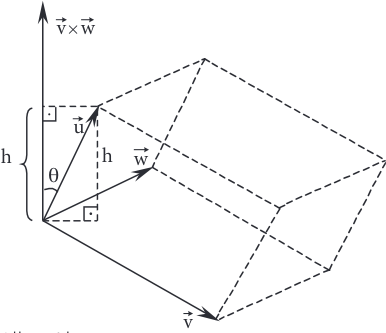
\includegraphics[width=0.5\textwidth]{./fig/fig4.3.png}\label{fig:fig4.3}
  \end{center}
\end{figure}

A área da base do paralelepípedo é dada por $|\vec{v} \times \vec{w}|$.

Seja $\theta$ o ângulo entre os vetores $\vec{u}$ e $\vec{v} \times \vec{w}$.
Sendo $\vec{v} \times \vec{w}$ um vetor ortogonal à base, a altura será paralela
a ele, e, portanto, a altura $h_u$ será dada por:
\[
  h_u = |\vec{v} \times \vec{w}| \cos \theta
\]
(É necessário considerar o valor absoluto $|\cos \theta|$, pois $\theta$ pode
ser um ângulo obtuso.)

Então, o volume $V$ do paralelepípedo é:
\[
  V = (\text{área da base})(\text{altura}) = |\vec{v} \times \vec{w}| \cdot |\cos \theta|
\]

Finalmente, o volume $V$ do paralelepípedo pode ser expresso como:
\[
  V = |(\vec{u}, \vec{v}, \vec{w})|
\]
no qual a última igualdade decorre da relação (2) do Produto Escalar.

\newpage
\subsection{Volume do Tetraedro}

Sejam $A$, $B$, $C$ e $D$ pontos não coplanares. Portanto, os vetores
$\overrightarrow{AB}$, $\overrightarrow{AC}$ e $\overrightarrow{AD}$ também são
não coplanares. Em consequência, esses vetores determinam um paralelepípedo
(Figura~\ref{fig:fig4.4}) cujo volume é dado por:

\[
  V_{\overrightarrow{AB}, \overrightarrow{AC}, \overrightarrow{AD}} = |(\overrightarrow{AB}, \overrightarrow{AC}, \overrightarrow{AD})|
\]

\begin{figure}[H]
  \begin{center}
    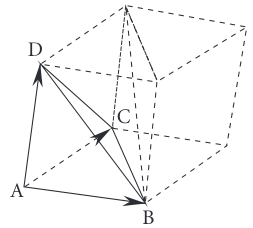
\includegraphics[width=0.5\textwidth]{./fig/fig4.4.png}\label{fig:fig4.4}
  \end{center}
\end{figure}

O paralelepípedo, por sua vez, pode ser repartido em dois prismas triangulares
de mesmo tamanho (conforme~\ref{fig:fig4.4}), e, portanto, o volume $V_p$ de
cada prisma é a metade do volume $V$ do paralelepípedo:

\[
  V_p = \frac{1}{2} V
\]

Por outro lado, da Geometria Espacial sabemos que o prisma pode ser repartido em
três pirâmides de mesmo volume, sendo uma delas o tetraedro $ABCD$. Assim, o
volume $V_t$ do tetraedro é um terço do volume do prisma, ou seja,

\[
  V_t = \frac{1}{3} V_p = \frac{1}{3} \cdot \frac{1}{2} V = \frac{1}{6} V
\]

Logo, o volume $V_t$ do tetraedro é dado por:

\[
  V_{\overrightarrow{AB}, \overrightarrow{AC}, \overrightarrow{AD}} = \frac{1}{6} |(\overrightarrow{AB}, \overrightarrow{AC}, \overrightarrow{AD})|
\]
